\chapter{Architektur}
Die Architektur unseres Projekts sieht an der Benutzeroberfl�che neben dem Navi-gations-Client einen Collector-Client und eine Admin-Oberfl�che vor. Die Informationen in einer zentralen Datenbank gespeichert und mit Hilfe eines Webservice bereitgestellt.

\begin{figure}[H]
\centering
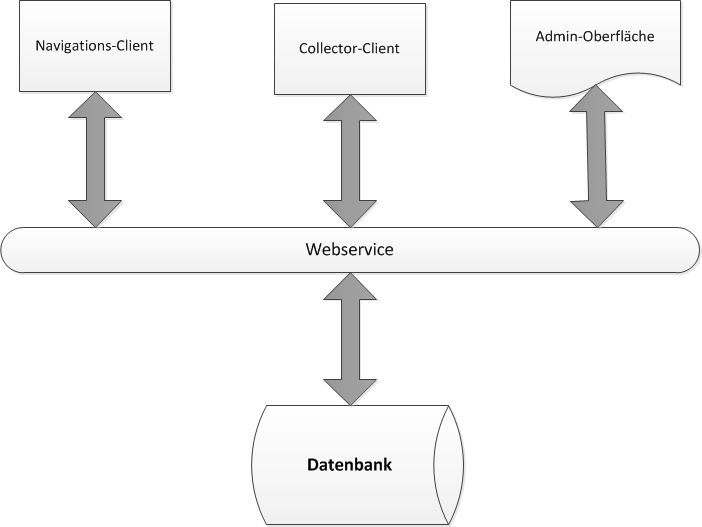
\includegraphics[width=\linewidth]{./Bilder/Architektur}
\caption{Grafische Darstellung der Architektur}
\label{fig:Achitektur}
\end{figure}

\section{Bestandteile}

Der \textbf{Navigations-Client} ist eine Anwendung f�r den Benutzers. Hier wird die Karte des Geb�udes mit allen Wegpunkten und die Navigation angezeigt. Dem Benutzer werden zus�tzlich zur Navigation Komfortfunktionen zur einfacheren und schnelleren Bedienung bereit gestellt.

Die \textbf{Admin-Oberfl�che} dient der Verwaltung von Karten und Benutzern. Der Administrator kann alte Karten bearbeiten oder neues Kartenmaterial einstellen. Zu diesen Karten wird auch der Graph mit allen Knoten und Kanten erstellt und anschlie�end verwaltet. Mit der Benutzerverwaltung k�nnen neue Benutzer angelegt und vorhandene bearbeitet werden oder aber alte Benutzerkonten gel�scht werden.

Mit dem \textbf{Collector-Client} soll der Datenbestand des Projektes fortlaufend erweitert werden. F�r die Knoten, bzw. Wegpunkte, k�nnen verschiedene, f�r die Navigation ben�tigte Informationen hinterlegt werden. Um fehlerhafte Eingaben zu vermeiden wird dieses Tool nicht vom Benutzer, sondern nur von Administratoren eingesetzt.

In der \textbf{Datenbank} werden s�mtliche Informationen der Anwendung gespeichert. Sie enth�lt die Benutzerdaten und das gesamte Kartenmaterial. Das Kartenmaterial umfasst dabei die Kartengrafiken wie auch den zugeh�rigen Graphen. �ber einen \textbf{Webservice} k�nnen die Daten abgerufen werden. Dieser stellt Funktionen zur Abfrage und Ablage von Navigations- und Benutzerdaten bereit.

Alternativ wurde uns ein Server mit einer �ffentlichen IP-Adresse an der Hochschule bereitgestellt, auf welchem das System jetzt betrieben wird.

\section{Kommunikation}
Die externen Kommunikation des Navigations-Clients, Collector-Clients und der Admin-Oberfl�che mit dem Webservice basiert auf HTTP. Als Austauschformat wird JSON verwendet.
Die interne Kommunikation des Webservices mit der Datenbank basiert auf dem Entity-Framework. 

Die westf�lische Hochschule hat einen Server mit einer festen IP-Adresse zur Verf�gung gestellt. Auf diesem betreiben wir einen IIS 7.5\footnote{\href{http://www.iis.net/}{http://www.iis.net/}} mit unserem Projekt.

